

\section{Convexity and optimisation}

\emph{Convexity} is perhaps the most important property that the elements forming an optimisation problem can present. Paraphrasing Tyrrell Rockafellar:

\begin{quote}
... in fact, the great watershed in optimization isn't between linearity and nonlinearity, but convexity and nonconvexity.
\end{quote}

The importance of convexity will become clear later in the course. In a nutshell, the existence of convexity allows us to infer global properties of a solution (i.e., that holds for all of its domain) by considering exclusively local information (such as gradients, for example). This is critical in the context of optimisation, since most of the methods we know to perform well in practice are designed to find solutions that satisfy local optimality conditions. Once convexity is attested, one can then guarantee that these local solutions are in fact globally optimal without exhaustively exploring the solution space. 

For a problem of the form
% 
\begin{align*}
    (P) :~ \mini & f(x) \\
    \st & x \in X
\end{align*}
%
to be convex, we need to verify whether $f$ is a \emph{convex function} and $X$ is a \emph{convex set}. If both statements hold true, we can conclude that $P$ is a \emph{convex problem}. We start looking into how to identify convex sets, since we can use the convexity of sets to infer the convexity of functions.


\section{Identifying convexity of sets}
 
Before we formally define convex sets, let us first look at the idea of \emph{combinations}. For that, let $S \subseteq \reals^n$ be a set and $x_j \in S$ for $j=1,\dots,k$ be a collection of vectors (i.e., $n$-dimensional ``points'') belonging to $S$. Then, we have that:
%
\begin{itemize} 
	\item A \emph{linear combination} of $x_j$ for $j=1,\dots, k$ is the set 
%
	\begin{align}
		\braces{x \in \reals^n : \sum_{j=1}^k \lambda_jx_j, \ \lambda_j \in \reals \text{ for } j=1,\dots, k}.
	\end{align}
%
	\item An \emph{affine combination} is a linear combination, with the additional constraint that $\sum_{j=1}^k \lambda_j = 1$. That is,
%
	\begin{align}
		\braces{x \in \reals^n : \sum_{j=1}^k \lambda_jx_j, \ \sum_{j=1}^k \lambda_j = 1, \ \lambda_j \in \reals \text{ for } j=1, \dots, k}.
	\end{align}
%
	\item A \emph{conic combination} is a linear combination with the additional condition that $\lambda_j \geq 0$ for $j = 1,\dots,k$.
%
	\begin{align}
		\braces{x \in \reals^n : \sum_{j=1}^k \lambda_jx_j, \ \lambda_j \geq 0 \text{ for } j=1,\dots,k}.
	\end{align}
%
	\item And finally, a \emph{convex combination} is the intersection between an affine and a conic combinations, implying that $\lambda_j \in [0,1]$.  
%
	\begin{align}
		\braces{x \in \reals^n : \sum_{j=1}^k \lambda_jx_j, \ \sum_{j=1}^k \lambda_j = 1, \ \lambda_j \geq 0 \text{ for } j=1,\dots,k}.
	\end{align}
% 
\end{itemize}

We say that a set is convex if it contains all points formed by the convex combination of any pair of points in this set. This is equivalent to saying that the set contains the line segment between any two points belonging to the set. 

\begin{definition}[Convex sets] \label{def:convex_sets}
	A set $S \subseteq \reals^n$ is said to be convex if $\overline{x} = \sum_{j=1}^k \lambda_jx_j$ belongs to $S$, where $\sum_{j=1}^k \lambda_j = 1$, $\lambda_j \geq 0$ and $x_j \in S$ for $j=1,\dots, k$.
\end{definition}

Definition \ref{def:convex_sets} is useful as it allows for showing that some set operations preserve convexity. 

\subsection{Convexity-preserving set operations}

\begin{lemma}[Convexity-preserving operations] \label{lem:convex_operations}
	Let $S_1$ and $S_2$ be convex sets in $\reals^n$. Then, the sets resulting from the following operations are also convex.
	\begin{enumerate}
		\item {Intersection:} $S = S_1 \cap S_2$;
		\item {Minkowski addition:} $S = S_1 + S_2 = \braces{x_1 + x_2 : x_1 \in S_1, x_2 \in S_2}$;
		\item {Minkowski\hspace{-1pt} difference:}\hspace{-2pt} $S = S_1 - S_2 = \braces{x_1 - x_2 : x_1 \in S_1, x_2 \in S_2}$;
		\item {Affine transformation:} $S = \braces{Ax + b : x \in S_1}$.
	\end{enumerate}
\end{lemma}

Figures \ref{fig:mink_sum} and \ref{fig:intersection} illustrate the concept behind some of these set operations. Showing that the sets resulting from the operations in Lemma \ref{lem:convex_operations} are convex typically entails showing that convex combinations of elements in the resulting set $S$ also belong to $S_1$ and $S_2$.

\begin{figure}
	\centering
    	\begin{tikzpicture}
%    		\draw[help lines] (-6,-3) grid (6,3);
    		\node (picture) at (0,0) {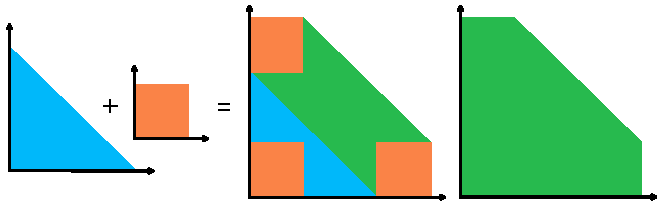
\includegraphics{part_2/chapter_2/figures/mink_sum}};
    		\node (A) at (-5, -0.5) {$S_1$};
    		\node (B) at (-2.9, -0.1) {$S_2$};
    		\node (C) at (-1, 1) {$S_2$};		
    		\node (D) at (-1, -1.1) {$S_2$};
    		\node (E) at (1.2, -1.1) {$S_2$};
    		\node (F) at (3, -0.5) {$S$};
    		\node (G) at (-1.1, -0.15) {$S_1$};
    	\end{tikzpicture}
		\caption{Minkowski sum of two convex sets.}\label{fig:mink_sum}
\end{figure}

%
\begin{figure}
	\centering
    \begin{tikzpicture}
%    		\draw[help lines] (-2,-2) grid (2,2);
    		\node (picture) at (0,0) {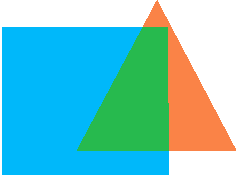
\includegraphics{part_2/chapter_2/figures/intersection.pdf}};
    		\node (A) at (-1, -0.15) {$S_1$};
    		\node (B) at (1.2, -0.5) {$S_2$};
    		\node (C) at (0.2, -0.8) {$S_1 \cap S_2$};
    \end{tikzpicture}
    
    \caption{Intersection of two convex sets.} \label{fig:intersection}
\end{figure}
%

\subsection{Examples of convex sets}

There are several familiar sets that are known to be convex. Having the knowledge that these sets are convex is useful as a building block for determining the convexity of more complicated sets.

Some important examples of convex sets include:
\begin{itemize}
	\item Them empty set $\emptyset$, any singleton $\{\overline{x}\}$ and the whole space $\reals^n$; 
	\item halfspaces: $S = \braces{x : p^\top x \leq \alpha} \subset \reals^n$;
	\item hyperplanes: $H = \braces{x : p^\top x = \alpha} \subset \reals^n$, where $p \neq 0^n$ is a normal vector and $\alpha\in \reals$ is a scalar. Notice that $H$ can be equivalently represented as $H = \braces{x \in \reals^n: p^\top(x - \overline{x}) = 0}$ for $\overline{x} \in H$;
	\item polyhedral sets: $P = \braces{x : Ax \leq b} \subset \reals^n$, where $A\in \reals^{m\times n}$ and $b \in \reals^n$;
	\item norm-induced sets (balls): $B = \braces{x : ||x - \overline{x}|| \leq \alpha} \subseteq \reals^n$, where $|| \cdot ||$ is any norm and $\alpha$ a scalar;
	\item norm cones: $C =\braces{(x,\alpha) \in \reals^{n+1}: ||x|| \leq \alpha} $;
\end{itemize} 

For example, let us consider the polyhedral set $P = \braces{x \in \reals^n : Ax \leq b} \subset \reals^n$ with $A$ being a $m \times n$ matrix. Notice that $S$ is the intersection of a collection of half-spaces $H_i = \braces{x \in \reals^n : a_i^\top x \leq b_i}$, where $a_i$ are vectors from the rows of the matrix $A$ and $b_i$ are the components of the column vector $b$. We know that $H_i$ are convex sets, thus $P = \cap_{i=1}^m H_i$ is also convex, as the intersection of sets is a convexity-preserving set operation.


\subsubsection{Hyperplanes and halfspaces}

Hyperplanes and halfspaces will play a central role in the developments we will see in our course. Therefore, let us take a moment and discuss some important aspects related these convex sets. First, notice that, geometrically, a hyperplane $H \subset \reals^n$ can be interpreted as the set of points with a \emph{constant} inner product to a given vector $p \in \reals^n$, while $\overline{x}$ determines the offset of the hyperplane from the origin. That is,
	\begin{equation*}
		H = \braces{x : p^\top(x - \overline{x}) = 0} \equiv \overline{x} + p^{\perp},
	\end{equation*}
	where $p^\perp$ is the orthogonal complement of $p$, i.e., the set of vectors orthogonal to $p$, which is given by $\braces{x \in \reals^n : p^\top x = 0}$.
	
	\begin{figure}[H]
	    \begin{tikzpicture}
%    		\draw[help lines] (-2,-2) grid (2,2);
    		\node (picture) at (0,0) {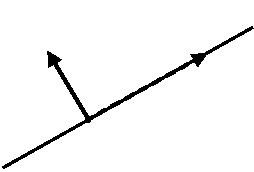
\includegraphics{part_2/chapter_2/figures/hyperplane.pdf}};
    		\node (p) at (-1.3, 0.8) {$p$};
    		\node (xbar) at (-0.6, -0.8) {$\overline{x}$};
    		\node (H) at (2, 0.5) {$H$};
		\end{tikzpicture}
		\caption{A hyperplane $H = \braces{x \in \reals^n: p^\top(x - \overline{x}) = 0}$ with normal vector $p$ displaced to $\overline{x}$.}
	\end{figure}
	
	Analogously, a halfspaces can be represented as $S = \braces{x \in \reals^n : p^\top(x - \overline{x}) \le 0}$ where $p^\top \overline{x} = \alpha$ is the hyperplane that forms the boundary of the halfspace. This definition suggests a simple geometrical interpretation: the halfspace $S$ consists of $\overline{x}$ plus any vector with an obtuse or right angle (i.e., greater of equal to 90$^\circ$) with the outward normal vector $p$.
 
 	\begin{figure}[H]
	    \begin{tikzpicture}
%    		\draw[help lines] (-2,-2) grid (2,2);
    		\node (picture) at (0,0) {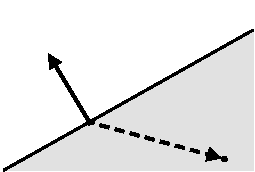
\includegraphics{part_2/chapter_2/figures/halfspace.pdf}};
    		\node (p) at (-1.3, 0.75) {$p$};
    		\node (xbar) at (-0.6, -0.9) {$\overline{x}$};
    		\node (x) at (1.9, -1.3) {$x$};
    		\node (H) at (1.7, 0.3) {$S$};
		\end{tikzpicture}
		\caption{A halfspace $S = \braces{x \in \reals^n : p^\top(x - \overline{x}) \le 0}$ defined by the same hyperplane $H$. Notice how the vectors $p$ (or $p - \overline{x}$, which is fundamentally the same vector but translated to $\overline{x}$) and $x - \overline{x}$ form angles greater or equal than $90^\circ$.}
	\end{figure}
	
	\begin{figure}[H]
    \begin{tikzpicture}
%    		\draw[help lines] (-2,-2) grid (2,2);
    		\node (picture) at (0,0) {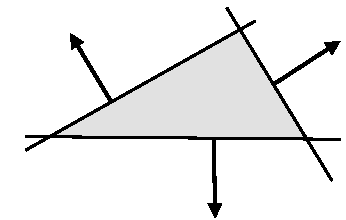
\includegraphics{part_2/chapter_2/figures/polyhedral_set.pdf}};
    		\node (P) at (0.75, 0.25) {$P$};
    		\node (a1) at (-1.6, 1.4) {$a_1$};
    		\node (a2) at (1, -1.8) {$a_2$};    		
    		\node (a2) at (2.8, 1.3) {$a_3$};
    \end{tikzpicture}
    \caption{A polyhedron $P$ formed by the intersection of three halfspace. Each hyperplane $H_i = \braces{x \in \reals^n : a_i^\top x \leq b_i}$, for $i = 1,2,3$, has a normal vector $a_i$, and has an offset from the origin $b_i$ (which cannot be seen once project on a 2-dimensional plane as in the picture).} \label{fig:polyhedral_set}
\end{figure}

\subsubsection{Norm balls and norm cones}

An Euclidean ball (or simply ball) of radius $\epsilon$ in $\reals^n$ has the form
%
\begin{equation*}
	B(\overline{x}, r) = \braces{x \in \reals^n : || x - \overline{x}||_2 \le \epsilon} \equiv \braces{x \in \reals^n : (x - \overline{x})^\top (x - \overline{x}) \le \epsilon^2}
\end{equation*}
%
As one might suspect, balls are convex, which can be proved by noting that
%
\begin{align*}
	||\lambda x_1 + (1 - \lambda) x_2 - \overline{x}||_2  & = ||\lambda (x_1 - \overline{x}) + (1 - \lambda) (x_2 - \overline{x})||_2 \\
	& \le \lambda ||x_1 - \overline{x}||_2 + + (1 - \lambda) ||x_2 - \overline{x}||_2 \le \epsilon.
\end{align*}
%
Notice that between the first and the second line, we use the triangle inequality, which states that $||x + y|| \le ||x|| + ||y||$ for any two vectors $x$ and $y$ and any norm (including the Euclidean norm). 

Euclidean balls are a special case of norm balls, which are defined as $B(\overline{x}, r) = \braces{x \in \reals^n : || x - \overline{x}|| \le \epsilon}$ where $||\ \cdot \ ||$ is any norm on $\reals^n$. 

A related set is the norm cone, defined as $C(x, \alpha) = \braces{(x,\alpha) \in \reals^{n+1} : ||x|| \le \alpha}$, where $\alpha$ is a scalar. For example, the second-order cone (also known as the ice cream cone or Lorentz cone) is the norm cone for the Euclidean norm.

\begin{remark} 
	Norm induced sets (balls or cones) are convex for any norm $||x||_p = \left(\sum_{i=1}^n x_i^p\right)^{\frac{1}{p}}$ for $x \in \reals^n$ and $p \geq 1$.
\end{remark}


\section{Convex hulls} 

A \emph{convex hull} of a set $S$, denoted $\conv(S)$ is the set formed by all convex combinations of all points in $S$. As the name suggests, $\conv(S)$ is a convex set, regardless of $S$ being or not convex. 

Another interpretation for $\conv(S)$ is to think of it as the tightest enveloping (convex) set that contains $S$. Notice that, if $S$ is convex, then $S = \conv(S)$.  Formally, convex hulls are defined as follows.

\begin{definition}[Convex hull of a set]\label{def: convex_hull}
	Let $S \subseteq \reals^n$ be an arbitrary set. The convex hull of $S$, denoted by $\conv(S)$, is the collection of all convex combinations of $S$. That is, for $x_j \in S$, with $j = 1,\dots, k$, $x \in \conv(S)$ if and only if 
	%
	\begin{equation*}
		x = \sum_{j=1}^k \lambda_jx_j : \sum_{j=1}^k \lambda_j = 1, \ \lambda_j \geq 0, \text{ for } j = 1,\dots,k.
	\end{equation*}                       
	%
\end{definition}
%

From Definition \ref{def: convex_hull}, one can show that the convex hull $\conv(S)$ can also be defined as the intersection of all convex sets containing $S$. Perhaps the easiest way to visualise this is to think of the infinitely many half-space containing $S$ and their intersection, which can only be $S$. Figure \ref{fig:convex_hull} illustrates the convex hull $\conv(S)$ of an nonconvex set $S$.
%
\begin{figure}[H]
%
\includegraphics[width=0.3\textwidth]{Figures/convex_hull.pdf}
	\begin{tikzpicture}
%    		\draw[help lines] (-3,-2) grid (3,2);
    		\node (picture) at (0,0) {
\includegraphics{part_2/chapter_2/figures/convex_hull.pdf}};
    		\node (A) at (-1.5, 0) {$S$};
    		\node (B) at (0.3, 0.5) {$\conv(S)$};
    \end{tikzpicture}
\caption{Example of an arbitrary set $S$ (in solid blue) and its convex hull $\conv(S)$ (combined blue and grey areas).} \label{fig:convex_hull}
\end{figure}
%
The notion of convex hulls is a powerful tool in optimisation. One important application is using $\conv(S)$ to obtain approximations for a nonconvex $S$ that can be exploited to solve an optimisation problem with constraint set defined by $S$. This is the underpinning technique in many important optimisation methods for such as branch-and-bound-based methods for nonconvex problems and decomposition methods (i.e., methods that solve large problems by breaking it into smaller parts that are presumably easier to solve).  

In specific, let us consider the convex hull of a finite collection of discrete points. Some of these sets are so important in optimisation that they have their own names. 
%
\begin{definition}
Let $S = \braces{x_1, \dots, x_{n+1}} \subset \reals^n$. Then $\conv(S)$ is called a \emph{polytope}. If $x_1,\dots,x_{n+1}$ are affinely independent (i.e., $x_2 - x_1, \dots ,x_{n+1} - x_1$ are linearly independent) then $\conv(S)$ is called a \emph{simplex} with vertices $x_1,\dots,x_{n+1}$.
\end{definition}
%


%\subsection{The Carath\'eodory theorem*}
%
%
%The \emph{Carath\'eodory theorem} is an important result associated with simplexes. It states that if $x \in \conv(S) \subset \reals^n$, then there exists a simplex composed by $x_j \in S$ for $j = 1, \dots, n+1$ that contains $x$. Formally, the theorem is posed as follows.
%%
%\begin{theorem}[Carath\'eodory theorem]
%Let $S \subseteq \reals^n$. If $x \in \conv(S)$, then $x \in \conv(x_1, \dots, x_{n+1})$ for some $x_j \in S$ where $j = 1,\dots, n+1$.        
%\end{theorem}   
%
%%% Consider including a proof for the Caratheodory theorem, for the sake of completeness.
%
%
%More specifically, any point $x \in \conv(S)$ can be expressed as
%%
%\begin{equation*}
%	x = \sum_{j=1}^{n+1} \lambda_jx_j : \sum_{j=1}^{n+1} \lambda_j = 1, \ \lambda_j \geq 0, \text{ for } j = 1,\dots,{n+1},
%\end{equation*}
%%
%for a given collection of points $x_j$, with $j = 1, \dots, n+1$ forming a simplex. Figure \ref{fig:caratheodory} illustrates this result.
%%
%\begin{figure}[h]
%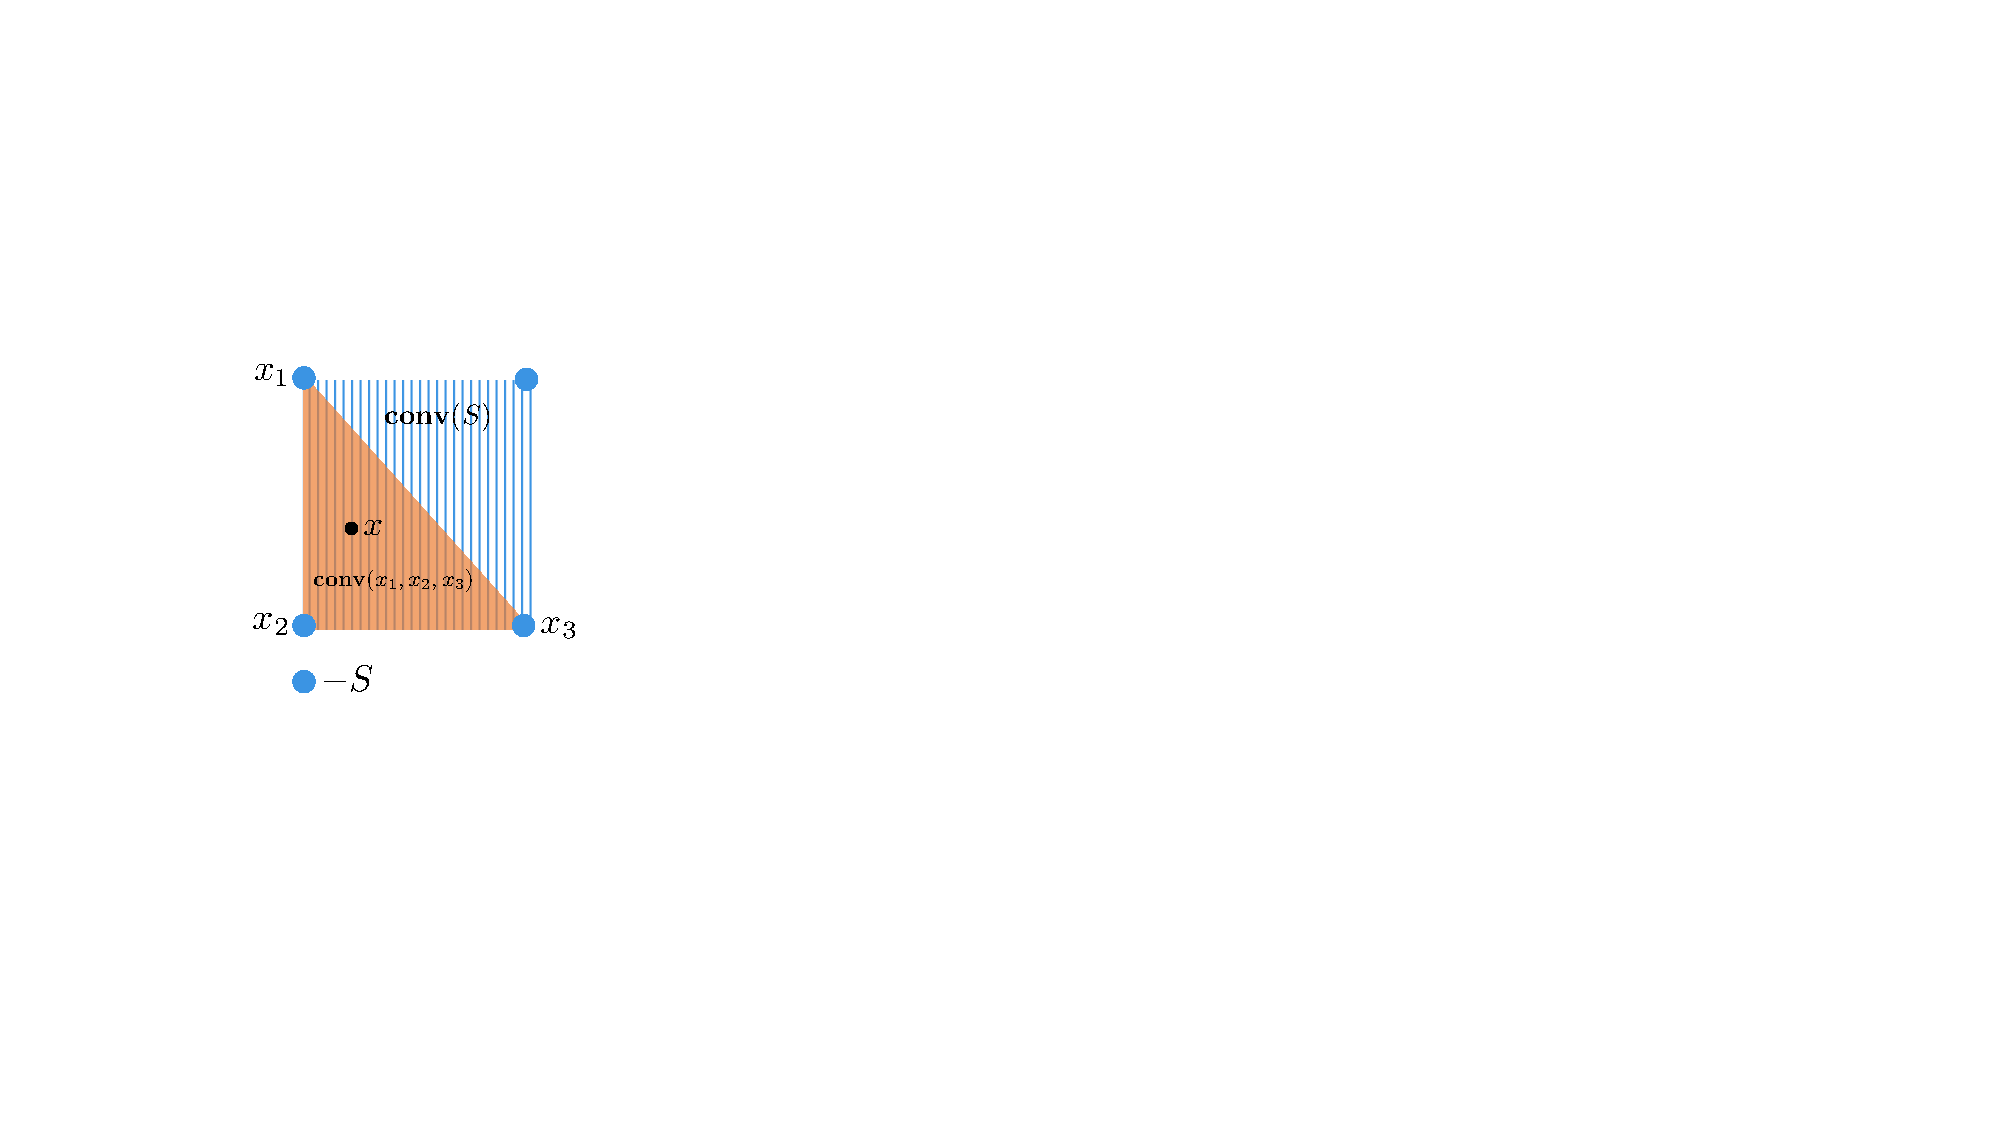
\includegraphics[width=0.3\textwidth]{Figures/caratheodory.pdf}
%\caption{Example of an arbitrary set $S$ (blue dots) and its convex hull $\conv(S)$ (light blue). Notice that $x$ can be represented as the convex combination of $x_j$ for $j=1,2,3$ for $n=2$.} \label{fig:caratheodory}
%\end{figure} 


\section{Closure and interior of sets}

Many of the set-related results we will see in this course depends on the characteristics of the set itself. Often, assuming properties such as closedness or compactness considerably ease technical derivations. 


\subsection{Closure, interior and boundary of a set}


Let us define some properties that will be useful in this course. For that, we will use an $\epsilon$-neighbourhood of $x \in \reals^n$ (which is a norm ball of radius $\epsilon$ centred in $x$) defined as
%
\begin{align*}
    N_\epsilon(x) = \braces{y : ||y - x|| < \epsilon}.
\end{align*}
%
Let $S \subseteq \reals^n$ be an arbitrary set. We can use $N_\epsilon$ to define the following elements related to $S$.  
\begin{enumerate}
\item \emph{Closure of $S$}: the set defined by the closure of $S$, denoted $\clo(S)$, is defined as 
%
\begin{align*}
\clo(S) = \braces{x \in \reals^n : S \cap N_\epsilon(x) \neq \emptyset \text{ for every } \epsilon > 0}. 
\end{align*}
%
Notice that the closure might contain points that do not belong to $S$. We say that a set is \emph{closed} if $S = \clo(S)$, that is, the set itself is its own closure. 
%
\item \emph{Interior of $S$}: the interior of $S$, denoted $\intr(S)$, is the set
\begin{align*}
\intr{S} = \braces{x \in S : N_\epsilon(x) \subset S \text{ for some } \epsilon > 0}.
\end{align*}
%
If $S$ is the same as its own interior, then we say that $S$ is \emph{open}. Some authors say that $S$ is solid if it has a nonempty interior (that is, $\intr(S) \neq \emptyset$. Notice that the interior of $S$ is a subset of $S$, that is $\intr(S) \subseteq S$.
%
\item \emph{Boundary of $S$}: the boundary of $S$, denoted $\bou(S)$ is the collection of points defined by
%
\begin{align*}
\bou(S) = \braces{x \in \reals^n : N_\epsilon(x) \text{ contains some } x_i \in S \text{ and some } x_j \notin S \text{ for every } \epsilon > 0}.
\end{align*}
%
We say that $S$ is bounded if exists $N_\epsilon(x)$, $x \in \reals^n$, for some $\epsilon > 0$ such that $S \subset N_\epsilon(x)$. 
\end{enumerate}

We say that a set is \emph{compact} if it is both \emph{closed} and \emph{bounded}. Compact sets appear very frequently in real-world applications of optimisation, since typically one can assume the existence of bounds for decision variables (such as nonnegativity or maximum physical bounds or, at an extreme case, smallest/ largest computational constants). Another frequent example of bounded set is the convex hull of a collection of discrete points, which is called by some authors \emph{polytopes} (effectively bounded polyhedral sets).  

Let us consider the following example. Let $S = \braces{(x_1,x_2) \in \reals^n : x_1^2 + x_2^2 \leq 1}$. Then, we have that:
\begin{enumerate}
	\item $\clo(S) = \braces{(x_1,x_2) \in \reals^n : x_1^2 + x_2^2 \leq 1}$. Since $S = \clo(S)$, $S$ is closed.
	\item $\intr(S) = \braces{(x_1,x_2) \in \reals^n : x_1^2 + x_2^2 < 1}$. 
	\item $\bou(S) = \braces{(x_1,x_2) \in \reals^n : x_1^2 + x_2^2 = 1}$. Notice that it makes $S$ bounded.
	\item $S$ is compact, since it is closed and bounded. 
\end{enumerate}

Notice that, if $S$ is closed, then $\bou(S) \subset S$. That is, its boundary is part of the set itself. Moreover, it can be shown that $\clo(S) = \bou(S) \cup S$ is the smallest closed set containing $S$. 

In case $S$ is convex, one can infer the convexity of the interior $\intr(S)$ and its closure $\clo(S)$. The following theorem summarises this result.
%
\begin{theorem}\label{thm:top_convex_comb}
Let $S \subseteq \reals^n$ be a convex set with $\intr(S) \neq \emptyset$. Let $x_1 \in \clo(S)$ and $x_2 \in \intr(S)$. Then $x = \lambda x_1 + (1 - \lambda) x_2 \in \intr(S)$ for all $\lambda \in (0,1)$.
\end{theorem}
%

% Consider including the proof for this theorem (on page 46)

Theorem \ref{thm:top_convex_comb} is useful for inferring the convexity of the elements related to $S$. We summarise the key results in the following corollary.
%
\begin{corollary} Let $S$ be a convex set with $\intr(S) \neq \emptyset$. Then
	\begin{enumerate}
		\item $\intr(S)$ is convex;
		\item $\clo(S)$ is convex;
		\item $\clo(\intr(S)) = \clo(S)$;
		\item $\intr(\clo(S)) = \intr(S)$.
	\end{enumerate}
\end{corollary}
%

% Consider including the proof for this corollary (on page 46)


\subsection{The Weierstrass theorem}


The Weierstrass theorem is a result that guarantees the existence of optimal solutions for optimisation problems. To make it more precise, let
%
\begin{align*}
	(P) :~ z = \mini\braces{f(x) : x \in S}  
\end{align*}
%
be our optimisation problem. If an optimal solution $x^*$ exists, then $f(x^*) \leq f(x)$ for all $x \in S$ and $z = f(x^*) = \min \braces{f(x) : x \in S}$. 

Notice the difference between $\mini$ (an abbreviation for minimise) and the operator $\min$. The first is meant to represent the problem of minimising the function $f$ in the domain $S$, while $\min$ is shorthand for minimum, in this case $z$, assuming that it is attainable.

It might be that an optimal solution is not attainable, but a bound can be obtained for the optimal solution value. The greatest lower bound for $z$ is its \emph{infimum} (or \emph{supremum} for maximisation problems), denoted by $\inf$. That is, if $z = \inf\braces{f(x) : x \in S}$ , then $z \leq f(x)$ for all $x \in S$ and there is no $\overline{z} > z$ such that $\overline{z} \leq f(x)$ for all $x \in S$. We might sometimes use the notation 
%
\begin{align*}
(P) :~ z = \inf\braces{f(x) : x \in S}
\end{align*}
%
to represent optimisation problems for which one cannot be sure whether an optimal solution is attainable. The Weierstrass theorem describes the situations in which those minimums (or maximums) are guaranteed to be attained, which is the case whenever $S$ is compact.
%
\begin{theorem}[Weierstrass theorem]\label{thm:weierstrass}
Let $S \neq \emptyset$ be a compact set, and let $f:S \rightarrow \reals$ be continuous on $S$. Then there exists a solution $\overline{x} \in S$ to $\mini\braces{f(x) : x \in S}$. 
\end{theorem}
%
Figure \ref{fig:Weierstrass} illustrates three examples. In the first (on the left) the domain $[a,b]$ is compact, and thus the minimum of $f$ is attained at $b$. In the other two, $[a,b)$ is open and therefore, Weierstrass theorem does not hold. In the middle example, one can obtain $\inf f$, which is not the case for the last example on the right.
%
\begin{figure}[h]
%\includegraphics[width=0.8\textwidth]{Figures/Weierstrass.pdf}
	\begin{tikzpicture}
%    		\draw[help lines] (-6,-1) grid (6,1);
    		\node (picture) at (0,0) {\includegraphics{part_2/chapter_2/figures/Weierstrass.pdf}};
    		\node (fa1) at (-5.8, 0.75) {$f(a)$};
    		\node (fb1) at (-5.8, -0.8) {$f(b)$};
 	    		\node (fa2) at (-1.8, 0.75) {$f(a)$};
    		\node (fb2) at (-1.8, -0.8) {$\inf f$};
 	    		\node (fa3) at (2.2, 0.75) {$f(a)$};
 	    		\node (a1) at (-5, -1.55) {$a$};
    		\node (b1) at (-3, -1.55) {$b$};
    		\node (a2) at (-1, -1.55) {$a$};
    		\node (b2) at (1, -1.55) {$b$};
 	    		\node (a3) at (3, -1.55) {$a$};
    \end{tikzpicture}
	\caption{Examples of attainable minimum (left) and infimum (centre) and an example where neither are attainable (right).} \label{fig:Weierstrass}
\end{figure}


\section{Separation and support of sets}
 

The concepts of \emph{separation} and \emph{support} of sets are key for establishing optimality conditions later in this course. We are interested in mechanisms that allow one to infer whether there exists hyperplanes separating points from sets (or sets from sets). We will also be interested in means to, given a point $x \notin S$, find the closest to point not belonging to $S$.

\subsection{Hyperplanes and closest points}

We start with how to identify closest points to sets. 
%
\begin{theorem}[Closest-point theorem]\label{thm:closest_point}
Let $S \neq \emptyset$ be a closed convex set in $\reals^n$ and $y \notin S$. Then, there exists a unique point $\overline{x} \in S$ with minimum distance from $y$. In addition, $\overline{x}$ is the minimising point if and only if $$(y-\overline{x})^\top(x - \overline{x}) \leq 0, \text{ for all } x\in S$$
\end{theorem}
%
Simply put, if $S$ is a closed convex set, then $\overline{x} \in S$ will be the closest point to $y \notin S$ if the vector $y - \overline{x}$ is such that if it forms an angle that is greater or equal than 90$^\circ$ with all other vectors $x - \overline{x}$ for $x \in S$. Figure \ref{fig:closest_point} illustrates this logic. 

\begin{figure}[h]
	\begin{tikzpicture}
%    	\draw[help lines] (-3,-2) grid (3,2);
		\node (picture) at (0,0) {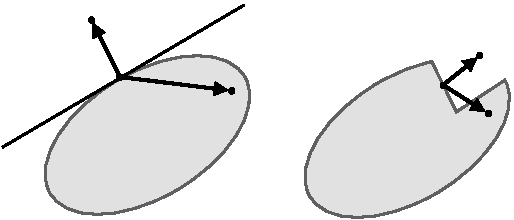
\includegraphics{part_2/chapter_2/figures/closest_point.pdf}};
		\node (y1) at (-2.8, 2) {$y$};
		\node (y2) at (4, 0.8) {$y$};
		\node (xbar1) at (-2.6, 0.4) {$\overline{x}$};
		\node (xbar2) at (2.9, 0.3) {$\overline{x}$};
		\node (x1) at (-0.4, -0.1) {$x$};    		
		\node (x2) at (3.9, -0.5) {$x$};
		\node (S) at (-2, -1) {$S$};
		\node (S) at (2, -1) {$S$};    		
    \end{tikzpicture}
	\caption{Closest-point theorem for a closed convex set (on the left). On the right, an illustration on how the absence of convexity invalidates the result.} \label{fig:closest_point}
\end{figure}

Notice that $S$ lies in the half-space $(y-\overline{x})^\top(x - \overline{x}) \leq 0$ defined by the hyperplane $p^\top(x - \overline{x}) =0$ with normal vector $p = (y - \overline{x})$. We will next revise the concepts of half-spaces and hyperplanes, since they will play a central role in the derivations in this course.  

\subsection{Halfspaces and separation}

We can use halfspaces to build the concept of separation. Let us start recalling that a hyperplane $H = \braces{x : p^\top x = \alpha}$ with normal vector $p \in \reals^n$ and $\alpha \in \reals$ defines two half-spaces $H^+ = \braces{x : p^\top x \geq \alpha}$ and $H^- = \braces{x : p^\top x \leq \alpha}$. Figure \ref{fig:hyperplane} illustrates the concept. Notice how the vector $p$ lies in the half-space $H^+$.
%
\begin{figure}
%	\includegraphics[scale=0.6]{Figures/hyperplanes.pdf}
	\begin{tikzpicture}
%    	\draw[help lines] (-2,-2) grid (2,2);
		\node (picture) at (0,0) {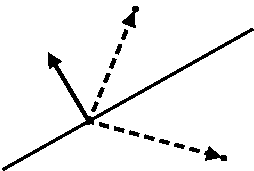
\includegraphics{part_2/chapter_2/figures/halfspaces.pdf}};
		\node (p) at (-1.4, 0.8) {$p$};
		\node (xbar) at (-0.7, -0.9) {$\overline{x}$};
		\node (H+) at (2, 1.2) {$H^{+}$};
		\node (H-) at (2, 0.5) {$H^{-}$};
	\end{tikzpicture}	
	\caption{Normal vectors, hyperplane and halfspaces} \label{fig:hyperplane}
\end{figure}
 
Any hyperplane $H$ can be defined in reference to a point $\overline{x} \in H$ by noticing that 
%
\begin{align*}
	p^\top(x - \overline{x}) = p^\top x - p^\top \overline{x} = \alpha - \alpha = 0.  
\end{align*}
%
From that, the half-spaces defined by $H$ can be equivalently stated as $H^+ = \braces{x : p^\top (x - \overline{x}) \geq 0}$ and $H^- = \braces{x : p^\top (x - \overline{x}) \leq 0}$.

We can now define the separation of convex sets. 
%
\begin{definition} \label{def:separation}
	Let $S_1$ and $S_2$ be nonempty sets in $\reals^n$. The hyperplane $H = \braces{x: p^\top x = \alpha}$ is said to \emph{separate} $S_1$ and $S_2$ if $ p^\top x \geq \alpha$ for each $x \in S_1$ and $p^\top x \leq \alpha$ for each $x \in S_2$. In addition, the following apply: 
	\begin{enumerate}
		\item {\bf Proper separation:} $S_1 \cup S_2 \not\subset H$;
		\item {\bf Strict separation:} $ p^\top x < \alpha$ for each $x \in S_1$ and $p^\top x > \alpha$ for each $x \in S_2$;
		\item {\bf Strong separation:} $ p^\top x \geq \alpha + \epsilon$ for some $\epsilon >0$ and $x \in S_1$, and $p^\top x \leq \alpha$ for each $x \in S_2$.
	\end{enumerate}
\end{definition}
%
Figure \ref{fig:separation} illustrates the three types of separation in Definition \ref{def:separation}. On the left, proper separation is illustrated, which is obtained by any hyperplane that does not contain both $S_1$ and $S_2$, but that might contain points from either or both. In the middle, sets $S_1$ and $S_2$ belong to two distinct half-spaces in a strict sense. On the right, strict separation holds with an additional margin $\epsilon > 0$, which is defined as strong separation. 
%
\begin{figure}[H]
%	\includegraphics[scale=0.8]{Figures/separations.pdf}
	\begin{tikzpicture}
%    	\draw[help lines] (-4,-2) grid (4,2);
		\node (picture) at (0,0) {\includegraphics{part_2/chapter_2/figures/separations.pdf}};
		\node (S11) at (-3.6, 0.5) {$S_1$};
		\node (S21) at (-3.15, -0.45) {$S_2$};
		\node (S12) at (-0.2, 0.5) {$S_1$};
		\node (S22) at (0.25, -0.45) {$S_2$};
		\node (S13) at (3, 0.5) {$S_1$};
		\node (S23) at (3.65, -0.45) {$S_2$};
		\node (H1) at (-2, 1.1) {$H$};		
		\node (H2) at (1.3, 1.1) {$H$};
		\node (H3) at (4.7, 1.1) {$H$};
	\end{tikzpicture}	
	\caption{Three types of separation between $S_1$ and $S_2$.} \label{fig:separation}
\end{figure}
%
A powerful yet simple result that we will use later is that, for a closed convex set $S$, there always exists a hyperplane separating $S$ and a point $y$ that does not belong to $S$.
%4
\begin{theorem}[Separation theorem]\label{thm:separation}
Let $S \neq \emptyset$ be a closed convex set in $\reals^n$ and $y \notin S$. Then, there exists a nonzero vector $p \in \reals^n$ and $\alpha \in \reals$ such that $p^\top x \leq \alpha$ for each $x \in S$ and $p^\top y > \alpha$.
\end{theorem}
%
\begin{proof}
	Theorem \ref{thm:closest_point} guarantees the existence of a unique minimising $\overline{x} \in S$ such that $(y-\overline{x})^\top(x - \overline{x}) \leq 0$ for each $x \in S$. Let $p = (y - \overline{x}) \neq 0$ and $\alpha = \overline{x}^\top(y - \overline{x}) = p^\top\overline{x}$. Then we get $p^\top x \leq \alpha$ for each $x \in S$, while $p^\top y - \alpha = (y - \overline{x})^\top(y - \overline{x}) = ||y - \overline{x}||^2 > 0$.
\end{proof}

This is the first proof we look at in these notes, and the reason for that is its importance in many of the results we will discuss further. The proof first looks at the problem of finding a minimum distance point as an optimisation problem and uses the Weierstrass theorem (our Theorem \ref{thm:closest_point} is a consequence of the Weierstrass theorem stated in Theorem \ref{thm:weierstrass}) to guarantee that such a $\overline{x}$ exists. Being a minimum distance point, we know from Theorem \ref{thm:closest_point} that $(y-\overline{x})^\top(x - \overline{x}) \leq 0$ holds. Now by defining $p$ and $\alpha$ as in the proof, one might notice that
%
\begin{align*}
	& (y-\overline{x})^\top(x - \overline{x}) \leq 0 \ \Leftrightarrow \ 
	(y-\overline{x})^\top x \leq (y - \overline{x})^\top\overline{x} \ \Leftrightarrow \ 
	p^\top x \leq p^\top\overline{x} = \alpha. 
\end{align*}
%
The inequality $p^\top y > \alpha$ is demonstrated to hold in the final part by noticing that 
%
\begin{align*}
	p^\top y - \alpha &= 
	(y - \overline{x})^\top y - \overline{x}^\top(y - \overline{x}) \\ &= 
	y^\top(y - \overline{x}) - \overline{x}^\top(y - \overline{x}) \\ & = (y - \overline{x})^\top (y - \overline{x}) = || y - \overline{x} ||^2 > 0.
\end{align*}

Theorem \ref{thm:separation} has interesting consequences. For example, one can apply it to every point in the boundary $\bou(S)$ to show that $S$ is formed by the intersection of all half-spaces containing $S$. 

Another interesting result is the existence of strong separation. If $y \notin \clo(\conv(S))$, then one can show that strong separation between $y$ and $S$ exists since there will surely be a distance $\epsilon>0$ between $y$ and $S$. 


\subsection{Farkas' theorem}

Farkas' theorem plays a central role in deriving optimality conditions. It can assume several alternative forms, which are typically referred to as Farkas' lemmas. In essence, the Farkas' theorem is used to demonstrate that a given system of linear equations has a solution if and only if a related system can be shown to have no solutions and vice-versa. 

\begin{theorem}
	Let $A$ be an $m \times n$ matrix and $c$ be an $n$-vector. Then exactly one of the following two systems has a solution:
	%
	\begin{align*}
		(1) :~ &Ax \leq 0, \ c^\top x > 0, \ x \in \reals^n\\
		(2) :~ &A^\top y = c, \ y \geq 0, \ y \in \reals^m.  
	\end{align*}
	%
\end{theorem}

\begin{proof}
	Suppose $(2)$ has a solution. Let $x$ be such that $Ax \leq 0$. Then $c^\top x = (A^\top y)^\top x = y^\top Ax \leq 0$. Hence, $(1)$ has no solution. 
	
	Next, suppose $(2)$ has no solution. Let $S = \braces{x \in \reals^n : x = A^\top y, \ y \geq 0}$. \hspace{-3pt}Notice that $S$ is closed and convex and that $c \notin S$. By Theorem \ref{thm:separation}, there exists $p \in \reals^n$ and $\alpha \in \reals$ such that $p^\top c > \alpha$ and $p^\top x \leq \alpha$ for $x \in S$. 
	
	As $0 \in S$, $\alpha \geq 0$ and $p^\top c > 0$. Also, $\alpha \geq p^\top A^\top y = y^\top Ap$ for $y \geq 0$. This implies that $Ap \leq 0$, and thus $p$ satisfies $(1)$. 
\end{proof}

The first part of the proof shows that, if we assume that system (2) has a solution, than $c^\top x > 0$ cannot hold for $y \geq 0$. The second part uses the separation theorem (Theorem \ref{thm:separation}) to show that $c$ can be seen as a point not belonging to the closed convex set $S$ for which there is a separation hyperplane and that the existence of such plane implies that system (1) must hold. The set $S$ is closed and convex since it is a conic combination of rows $a_i$, for $i=1, \dots, m$. Using the $0 \in S$, one can show that $\alpha \geq 0$. The last part uses the identity $p^\top A^\top  = (Ap)^\top$ and the fact that $(Ap)^\top y = y^\top Ap$. Notice that, since $y$ can be arbitrarily large and $\alpha$ is a constant, $y^\top Ap \leq \alpha$ can only hold if $y^\top Ap \leq 0$, requiring that $p \leq 0$ since $y \geq 0$ from the definition of $S$.

Farkas' theorem has an interesting geometrical interpretation arising from this proof, as illustrated in Figure \ref{fig:farkas}. Consider the cone $C$ formed by the rows of $A$
%
\begin{align*} 
	C = \braces{c \in \reals^n : c_j = \sum_{i=1}^m a_{ij} y_i, \ j= 1,\dots,n, \  y_i \geq 0, \ i =1,\dots, m}
\end{align*}
%
The \emph{polar cone} of $C$, denoted $C^0$, is formed by the all vectors having angles of 90$^\circ$ or more with vectors in $C$. That is, 
%
\begin{align*}
	C^0 = \braces{x : Ax \leq 0}.
\end{align*}
%
Notice that $(1)$ has a solution if the intersection between the polar cone $C^0$ and the positive ($H^+$ as defined earlier) half-space $H^+ = \braces{x \in \reals^n: c^\top x > 0}$ is not empty. If $(2)$ has a solution, as in the beginning of the proof, then $c \in C$ and the intersection $C^0 \cap H^+ = \emptyset$. Now, if $(2)$ does not have a solution, that is, $c \notin C$, then one can see that $C^0 \cap H^+$ cannot be empty, meaning that $(1)$ has a solution.  

\begin{figure}[h]
%	\includegraphics[width = 0.7\textwidth]{Figures/farkas.pdf}
	\begin{tikzpicture}
%    	\draw[help lines] (-5,-2) grid (5,2);
		\node (picture) at (0,0) {\includegraphics{part_2/chapter_2/figures/farkas.pdf}};
		\node (C01) at (-4,-0.5) {$C_0$};
		\node (C01) at (1.5,-0.7) {$C_0$};
		\node (C1) at (-1.5,-0.5) {$C$};
		\node (C2) at (4,-0.5) {$C$};
		\node (c1) at (-1.4,0) {$c$};
		\node (c2) at (2,1.7) {$c$};			
		\node (a11) at (-1.7,2) {$a_1$};
		\node (a12) at (3.8,2) {$a_1$};
		\node (a21) at (-0.8,1) {$a_2$};
		\node (a12) at (4.7,1) {$a_2$};
		\node (a31) at (-0.4,-1.3) {$a_3$};
		\node (a31) at (5.1,-1.3) {$a_3$};
	\end{tikzpicture}
	\caption{Geometrical illustration of the Farkas' theorem. On the left, system $(2)$ has a solution, while on the right, system $(1)$ has a solution} \label{fig:farkas}
\end{figure}


\subsection{Supporting hyperplanes}

There is an important connection between the existence of hyperplanes that support a whole set and optimality conditions of points. Let us first define supporting hyperplanes. 

\begin{definition}[Supporting hyperplane]
	Let $S \neq \emptyset$ be a set in $\reals^n$, and let $\overline{x} \in \bou(S)$. $H = \braces{x \in \reals^n : p^\top (x-\overline{x}) =0}$ is a supporting hyperplane of $S$ at $\overline{x}$ if either $S \subseteq H^+$ (i.e., $p^\top (x-\overline{x}) \geq 0$ for $x \in S$) or $S \subseteq H^-$.  
\end{definition}

Figure \ref{fig:support_hyperplane} illustrates the concept of supporting hyperplanes. Notice that supporting hyperplanes might not be unique, with the geometry of the set $S$ playing an important role in that matter. 

Let us define the function $f(x) = p^\top x$ with $x \in S$. One can see that the optimal solution $\overline{x}$ given by 
%
\begin{align*}
	\overline{x} = \argmax_{x \in S} f(x)
\end{align*}
%
is a point $x \in S$ for which $p$ is a supporting hyperplane. A simple geometric analogy is to think that the $f$ increases value as one moves in the direction of $p$. The constraint $x \in S$ will eventually prevent the movement further from $S$ and this last contact point is precisely $\overline{x}$. This is a useful concept for optimising problem using gradients of functions, as we will discuss later in the course.

\begin{figure}[h]
	%\includegraphics[width=0.9\textwidth]{Figures/support_hyperplane.pdf}
	\begin{tikzpicture}
%    	\draw[help lines] (-6,-2) grid (6,2);
		\node (picture) at (0,0) {\includegraphics{part_2/chapter_2/figures/support_hyperplane.pdf}};
		\node (S1) at (-4.3,-0.5) {$S$};
		\node (S2) at (-1,-0.5) {$S$};
		\node (S3) at (2.5,-0.5) {$S$};
		\node (xbar1) at (-3.6,-0.5) {$\overline{x}$};
		\node (xbar2) at (0.55,0.35) {$\overline{x}$};
		\node (p11) at (-3, -1.5) {$p$};		
		\node (p21) at (1.4, 0.75) {$p_1$};		
		\node (p22) at (1.6, 0.3) {$p_2$};
		\node (p31) at (4.3, 1.4) {$p$};
		\node (p32) at (5.05, 0.6) {$p$};
		\node (xbar31) at (3.52, 0.57) {$\overline{x}_1$};				
		\node (xbar32) at (4.25, -0.2) {$\overline{x}_2$};						
	\end{tikzpicture}
	\caption{Supporting hyperplanes for an arbitrary set. Notice how a single point might have multiple supporting planes (middle) or different points might have the same supporting hyperplane (right)} \label{fig:support_hyperplane} 
\end{figure}

One characteristic that convex sets present that will be of great importance when establishing optimality conditions is the existence of supporting hyperplanes at every boundary point.

\begin{theorem}[Support of convex sets]
	Let $S \neq \emptyset$ be a convex set in $\reals^n$, and let $\overline{x} \in \bou(S)$. Then there exists $p \neq 0$ such that $p^\top(x - \overline{x}) \leq 0$ for each $x \in \clo(S)$.
\end{theorem}

The proof follows immediately from Theorem \ref{thm:separation}, without explicitly considering a point $y \notin S$ and by noticing that $\bou(S) \subset \clo(S)$. Figure \ref{fig:support_convex} provides an illustration of the theorem. 

\begin{figure}[H]
%	\includegraphics[width=0.3\textwidth]{Figures/support_convex.pdf}
	\begin{tikzpicture}
%    	\draw[help lines] (-2,-2) grid (2,2);
		\node (picture) at (0,0) {\includegraphics{part_2/chapter_2/figures/support_convex.pdf}};
		\node (S) at (0.25,-0.5) {$S$};
		\node (S) at (-1,1.6) {$p$};
		\node (S) at (1.6, -0.1) {$\overline{x}$};
	\end{tikzpicture}
	\caption{Supporting hyperplanes for convex sets. Notice how every boundary point has at least one supporting hyperplane} \label{fig:support_convex}
\end{figure}

